\chapter{Kiểm thử, đánh giá và hướng phát triển}\label{chap:evaluation}

Chương này trình bày chiến lược kiểm thử, kết quả kiểm thử chức năng, bảo mật, giao diện và gợi ý, rồi đánh giá mô hình LightGBM cùng giới hạn của dữ liệu trước phát hành. Phần cuối đánh giá tổng thể hệ thống và đề xuất hướng phát triển. Mọi kết quả trong chương được lấy từ nhật ký chạy kiểm thử ngày 24--25/10/2026. Các thực nghiệm có ghi dữ liệu chỉ chạy trên cơ sở dữ liệu cục bộ, không chạy trên môi trường vận hành.

\section{Chiến lược kiểm thử}\label{sec:test-strategy}

\Cref{tab:test-levels} mô tả các mức kiểm thử, công cụ, phạm vi và số lượng ca. Kiểm thử đơn vị và tích hợp chạy tự động mỗi khi thay đổi mã. Kiểm thử trên MongoDB thật cần một replica set riêng nên chạy theo lệnh. Kiểm thử giao diện và kiểm thử đầu-cuối được thực hiện thủ công trên Simulator và trình duyệt, với dữ liệu tạo qua chính API của hệ thống.

\begin{rtable}
\begin{longtable}{|L{2.9cm}|L{3.5cm}|L{5.4cm}|C{2.8cm}|}
\caption{Các mức kiểm thử}\label{tab:test-levels}\\
\hline
\thead{Mức} & \thead{Công cụ} & \thead{Phạm vi} & \thead{Số ca, kết quả} \\ \hline
\endfirsthead
\hline
\thead{Mức} & \thead{Công cụ} & \thead{Phạm vi} & \thead{Số ca, kết quả} \\ \hline
\endhead
Đơn vị (máy chủ) & Jest 30, ts-jest & Quy tắc ngày, tồn kho, máy trạng thái, xác thực, webhook, bộ xếp hạng, cấu hình & 57 ca / 14 bộ; 57 đạt \\ \hline
Tích hợp dịch vụ (máy chủ) & Jest với MongoDB giả lập trong bộ nhớ & BookingsService, PaymentsService, RecommendationsService, luồng trả tại khách sạn & (nằm trong 57 ca) \\ \hline
Tích hợp cơ sở dữ liệu thật & Node, MongoDB 7.0 replica set (Docker) & Tranh chấp, thử lại, hết hạn, hủy, nhận/trả phòng & 1 kịch bản, 24 khẳng định; đạt \\ \hline
Đơn vị (nghiên cứu ML) & pytest 9.1 & Đặc trưng Python, chuẩn hóa, giờ Việt Nam, ảnh chụp danh mục, pipeline Trivago & 80 ca; 80 đạt \\ \hline
Phân quyền qua HTTP & Kịch bản Node gọi API cục bộ & Vai trò, quyền sở hữu, loại token, kiểm tra đầu vào, thu hồi phiên & 13 + 7 ca; 20 đạt \\ \hline
Khả năng chịu lỗi của mô hình & Kịch bản Node trên bản sao thư mục build & Tệp mô hình hỏng, thiếu, sai đặc trưng & 6 kịch bản; 6 đạt \\ \hline
Giao diện iOS & iOS Simulator, iPhone 17 Pro & Luồng khách đầy đủ, tiếng Việt và tiếng Anh & 18 ca thủ công (\cref{tab:test-ui}) \\ \hline
Giao diện web & Chrome headless (Puppeteer) & 14 trang owner/admin; 3 kích thước màn hình; lỗi console, HTTP, tràn ngang & 16 ảnh; 0 lỗi tự động phát hiện \\ \hline
Kiểm tra trên môi trường vận hành & curl, dig & Sức khỏe API, phiên bản mô hình, DNS & chỉ đọc \\ \hline
\end{longtable}
\end{rtable}

Hệ thống chưa có kiểm thử giao diện tự động (XCUITest, Playwright), chưa có kiểm thử tải và chưa có kiểm thử với cổng payOS thật. Đây là các giới hạn được nêu ở \cref{sec:limitations}.

\section{Kiểm thử chức năng đặt phòng}\label{sec:test-booking}

\subsection{Kiểm thử tự động}

\Cref{tab:test-booking} là các ca kiểm thử của luồng đặt phòng. Các ca TC-B chạy bằng Jest với cơ sở dữ liệu giả lập. Các ca TC-D chạy trên MongoDB thật với giao dịch thật, nhằm loại trừ khả năng mô hình giả lập che khuất lỗi đồng thời.

\begin{rtable}
\begin{longtable}{|C{1.4cm}|L{6.6cm}|L{5.0cm}|C{1.6cm}|}
\caption{Ca kiểm thử luồng đặt phòng}\label{tab:test-booking}\\
\hline
\thead{Mã} & \thead{Kịch bản} & \thead{Kết quả mong đợi} & \thead{Kết quả} \\ \hline
\endfirsthead
\hline
\thead{Mã} & \thead{Kịch bản} & \thead{Kết quả mong đợi} & \thead{Kết quả} \\ \hline
\endhead
TC-B01 & Nhận phòng hôm nay theo giờ Việt Nam; tính số đêm & Hợp lệ; số đêm đúng theo \cref{eq:nights} & Đạt \\ \hline
TC-B02 & Ngày đảo ngược, không hợp lệ, ở quá khứ, quá 90 đêm & Từ chối 400 & Đạt \\ \hline
TC-B03 & Đặt phòng [10, 12) và [12, 14) với 1 phòng; đếm theo từng đêm & Không chồng lấn; ngày trả không chiếm tồn kho & Đạt \\ \hline
TC-B04 & Đặt phòng CONFIRMED và giữ chỗ đã hết hạn & CONFIRMED chiếm tồn kho; giữ chỗ hết hạn thì không & Đạt \\ \hline
TC-B05 & Giữ phòng không xác nhận quá 15 phút & Chuyển EXPIRED, giải phóng phòng & Đạt \\ \hline
TC-B06 & Gửi lại cùng khóa, cùng nội dung; cùng khóa, khác nội dung & Trả lại đặt phòng cũ; 409 & Đạt \\ \hline
TC-B07 & Hai khách cùng đặt căn phòng cuối & Đúng một khách thành công & Đạt \\ \hline
TC-B08 & Đặt khách sạn thuộc danh mục chỉ xem dù đã có loại phòng & Từ chối & Đạt \\ \hline
TC-B09 & Hủy đặt phòng CONFIRMED & CANCEL\_REQUESTED, vẫn giữ tồn kho tới khi chủ khách sạn xác nhận & Đạt \\ \hline
TC-B10 & Giữ phòng, thử lại, trả tại khách sạn, nhận phòng, trả phòng & Chuỗi trạng thái đúng; thao tác lặp lại lũy đẳng & Đạt \\ \hline
TC-D01 & MongoDB thật: hai khách gửi đồng thời (\code{Promise.allSettled}) cho loại phòng còn 1 phòng & 1 thành công; tổng số đặt phòng = 1 & Đạt \\ \hline
TC-D02 & MongoDB thật: gửi lại cùng khóa; hai yêu cầu cùng khóa đồng thời; cùng khóa khác nội dung & Cùng một đặt phòng; không tạo thêm; lỗi ``nội dung khác'' & Đạt \\ \hline
TC-D03 & MongoDB thật: giữ phòng hết hạn; gửi lại khóa cũ; xác nhận trả tại khách sạn sau khi hết hạn & Trả về EXPIRED; từ chối xác nhận & Đạt \\ \hline
TC-D04 & MongoDB thật: hủy giữ chỗ; xác nhận rồi hủy; đặt lại trước và sau khi chủ khách sạn xác nhận hủy & Phòng bị giữ khi CANCEL\_REQUESTED; trống lại sau khi CANCELLED & Đạt \\ \hline
TC-D05 & MongoDB thật: người không sở hữu nhận phòng; chủ khách sạn nhận/trả phòng hai lần; đặt chồng ngày lưu trú & 403; lũy đẳng; hết phòng & Đạt \\ \hline
\end{longtable}
\end{rtable}

\Cref{lst:dblog} là nhật ký chạy kịch bản trên MongoDB thật. Kịch bản tạo một cơ sở dữ liệu mới với tên ngẫu nhiên cho mỗi lần chạy và xóa nó khi kết thúc.

\begin{lstlisting}[caption={Nhật ký kiểm thử tranh chấp trên MongoDB 7.0 replica set}, label={lst:dblog}, numbers=none]
Sat Oct 24 21:53:54 +07 2026
> hotelia-api@1.0.0 test:booking-db
> node scripts/test-booking-concurrency.cjs
PASS: contention, retry, expiry, cancellation, pay-at-hotel, owner check-in/out
      and occupied stay dates.
\end{lstlisting}

\subsection{Hết thời gian chờ và thử lại}

Lỗi mạng giữa ứng dụng và máy chủ khó tái hiện tự động. Đồ án kiểm chứng tình huống này theo hai lớp. Phía máy chủ, TC-D02 xác nhận rằng một yêu cầu gửi lại với cùng khóa, kể cả khi hai yêu cầu đến đồng thời, chỉ tạo một đặt phòng. Phía ứng dụng, mã nguồn ở \cref{lst:bookroom} cho thấy khóa được giữ nguyên khi lỗi thuộc loại không xác định. Hai lớp kết hợp bảo đảm rằng việc khách bấm ``Kiểm tra lại kết quả'' sau khi hết thời gian chờ không tạo đặt phòng thứ hai. Đồ án chưa có kiểm thử đầu-cuối tự động mô phỏng mất kết nối đúng lúc máy chủ vừa ghi xong; đây là ca nên bổ sung bằng công cụ chặn mạng (ví dụ proxy có độ trễ).

\subsection{Kiểm thử thủ công trên ứng dụng}

Luồng đặt phòng được thực hiện đầy đủ trên Simulator với máy chủ cục bộ (\cref{fig:scr-booking,fig:scr-payment}): chọn Rex Hotel Saigon, loại phòng Deluxe, 1 đêm; ứng dụng hiển thị ``Đã giữ phòng'' kèm hạn giữ; chọn ``Thanh toán tại khách sạn'' và đặt phòng chuyển sang ``Đã xác nhận''. Một đặt phòng giữ chỗ khác không được xác nhận đã tự chuyển sang ``Hết hạn'' sau 15 phút (\cref{fig:scr-english}c). Các trạng thái đã nhận phòng, đã trả phòng, yêu cầu hủy và đã hủy được tạo qua API bằng tài khoản chủ khách sạn rồi kiểm tra trên ứng dụng (\cref{fig:scr-account}a).

\section{Kiểm thử xác thực, phân quyền, thanh toán và quản trị}\label{sec:test-auth}

\subsection{Xác thực}

\Cref{tab:test-auth} là các ca kiểm thử tự động của xác thực và cấu hình bảo mật. TC-A05 đến TC-A08 được bổ sung khi sửa lỗi refresh token dùng được như access token; TC-A13 đến TC-A17 được bổ sung khi sửa cách lưu và thu hồi refresh token (\cref{sec:impl-auth}).

\begin{rtable}
\begin{longtable}{|C{1.4cm}|L{8.0cm}|L{3.6cm}|C{1.6cm}|}
\caption{Ca kiểm thử xác thực và cấu hình}\label{tab:test-auth}\\
\hline
\thead{Mã} & \thead{Kịch bản} & \thead{Mong đợi} & \thead{Kết quả} \\ \hline
\endfirsthead
\hline
\thead{Mã} & \thead{Kịch bản} & \thead{Mong đợi} & \thead{Kết quả} \\ \hline
\endhead
TC-A01 & ID token sai chữ ký, sai \code{aud} hoặc hết hạn & 401, không tạo người dùng & Đạt \\ \hline
TC-A02 & ID token Google hợp lệ, email đã xác minh & Tạo phiên Hotelia & Đạt \\ \hline
TC-A03 & Email Google chưa xác minh hoặc không có thẩm quyền & Không liên kết theo email & Đạt \\ \hline
TC-A04 & Nonce Apple không khớp lần đăng nhập & 401 & Đạt \\ \hline
TC-A05 & Ký access và refresh token & \code{typ} khác nhau & Đạt \\ \hline
TC-A06 & Dùng access token để làm mới phiên & 401 & Đạt \\ \hline
TC-A07 & JwtStrategy với access token & Chấp nhận & Đạt \\ \hline
TC-A08 & JwtStrategy với refresh token & Từ chối & Đạt \\ \hline
TC-A09 & Cấu hình phát triển hợp lệ & Khởi động & Đạt \\ \hline
TC-A10 & Thiếu \code{MONGODB\_URI} hoặc \code{JWT\_SECRET} & Từ chối khởi động & Đạt \\ \hline
TC-A11 & \code{JWT\_SECRET} dạng mẫu ở môi trường vận hành & Từ chối khởi động & Đạt \\ \hline
TC-A12 & Môi trường vận hành không khai báo \code{CORS\_ORIGINS} & Từ chối khởi động & Đạt \\ \hline
TC-A13 & Hai refresh token của cùng người dùng (giống nhau ở 72 byte đầu); xoay vòng sang token mới & Token cũ bị từ chối & Đạt \\ \hline
TC-A14 & Thu hồi phiên rồi dùng lại refresh token & Từ chối & Đạt \\ \hline
TC-A15 & Bản băm bcrypt lưu trước bản sửa & Vẫn chấp nhận tới lần xoay vòng kế tiếp & Đạt \\ \hline
TC-A16 & Đăng xuất bằng refresh token hợp lệ & Xóa bản băm phiên & Đạt \\ \hline
TC-A17 & Đăng xuất bằng access token, token cũ hoặc token giả & Trả cùng thông báo, không thu hồi & Đạt \\ \hline
\end{longtable}
\end{rtable}

\subsection{Phân quyền qua HTTP}

\Cref{tab:test-authz} là kết quả gọi API thật trên máy chủ cục bộ bằng ba tài khoản thử nghiệm USER, OWNER và ADMIN. Ca A10 ban đầu cho kết quả 403 thay vì 200. Nguyên nhân là kịch bản chọn nhầm một đặt phòng thuộc khách sạn mà chủ khách sạn thử nghiệm không sở hữu, nên 403 là phản hồi đúng. Sau khi sửa dữ liệu của kịch bản, ca này đạt; tình huống bị chọn nhầm được giữ lại thành ca A13.

\begin{rtable}
\begin{longtable}{|C{1.0cm}|L{7.6cm}|C{1.6cm}|C{1.6cm}|C{1.8cm}|}
\caption{Ca kiểm thử phân quyền qua API}\label{tab:test-authz}\\
\hline
\thead{Mã} & \thead{Kịch bản} & \thead{Mong đợi} & \thead{Thực tế} & \thead{Kết quả} \\ \hline
\endfirsthead
\hline
\thead{Mã} & \thead{Kịch bản} & \thead{Mong đợi} & \thead{Thực tế} & \thead{Kết quả} \\ \hline
\endhead
A1 & Không có token gọi \code{GET /bookings} & 401 & 401 & Đạt \\ \hline
A2 & USER gọi \code{GET /admin/stats} & 403 & 403 & Đạt \\ \hline
A3 & OWNER gọi \code{GET /admin/users} & 403 & 403 & Đạt \\ \hline
A4 & ADMIN gọi \code{GET /admin/stats} & 200 & 200 & Đạt \\ \hline
A5 & USER gọi nhận phòng & 403 & 403 & Đạt \\ \hline
A6 & USER gọi \code{GET /owners/revenue} & 403 & 403 & Đạt \\ \hline
A7 & OWNER xem đặt phòng của khách sạn không sở hữu qua \code{/owners/hotels/:id/bookings} & 404 & 404 & Đạt \\ \hline
A8 & Refresh token dùng làm Bearer & 401 & 401 & Đạt \\ \hline
A9 & Access token gửi tới \code{/auth/refresh} & 401 & 401 & Đạt \\ \hline
A10 & OWNER xem chi tiết đặt phòng tại khách sạn của mình & 200 & 200 & Đạt \\ \hline
A11 & Gửi trường \code{role} khi cập nhật hồ sơ & 400 & 400 & Đạt \\ \hline
A12 & Webhook payOS không có chữ ký & 400 & 400 & Đạt \\ \hline
A13 & OWNER xem chi tiết đặt phòng tại khách sạn không sở hữu & 403 & 403 & Đạt \\ \hline
\end{longtable}
\end{rtable}

Ca A11 cho thấy \code{ValidationPipe} với \code{forbidNonWhitelisted} chặn tấn công gán hàng loạt (mass assignment): người dùng không thể tự nâng vai trò bằng cách gửi thêm trường \code{role}.

\subsection{Phiên đăng nhập}

\Cref{tab:test-session} kiểm tra việc xoay vòng và thu hồi refresh token, cùng chức năng xóa lịch sử gợi ý, trên cùng máy chủ cục bộ. Lần chạy đầu, ca S2 không đạt: lần đăng nhập và lần làm mới diễn ra trong cùng một giây nên máy chủ phát lại đúng refresh token cũ. Sau khi thêm claim \code{jti} ngẫu nhiên, cả bảy ca đều đạt.

\begin{rtable}
\begin{longtable}{|C{1.0cm}|L{11.0cm}|C{1.8cm}|}
\caption{Ca kiểm thử phiên đăng nhập và xóa lịch sử gợi ý}\label{tab:test-session}\\
\hline
\thead{Mã} & \thead{Kịch bản} & \thead{Kết quả} \\ \hline
\endfirsthead
\hline
\thead{Mã} & \thead{Kịch bản} & \thead{Kết quả} \\ \hline
\endhead
S1 & Làm mới phiên bằng refresh token hiện tại & Đạt \\ \hline
S2 & Refresh token cũ bị từ chối sau khi xoay vòng & Đạt \\ \hline
S3 & Đăng xuất chỉ với refresh token (không có access token) trả 200 & Đạt \\ \hline
S4 & Refresh token đã thu hồi không làm mới được phiên & Đạt \\ \hline
S5 & Đăng xuất với token giả vẫn trả 200, không lộ thông tin & Đạt \\ \hline
S6 & Gửi access token tới \code{/auth/logout} không thu hồi phiên & Đạt \\ \hline
S7 & Sau khi xóa lịch sử gợi ý, gợi ý không còn được cá nhân hóa & Đạt \\ \hline
\end{longtable}
\end{rtable}

\subsection{Thanh toán và webhook}

\Cref{tab:test-pay} là các ca kiểm thử của thanh toán. TC-P05 và TC-P06 dùng chính thư viện payOS để ký một webhook bằng khóa thử nghiệm. TC-P06 xác nhận rằng nếu kẻ tấn công sửa số tiền nhưng giữ nguyên chữ ký cũ, webhook bị từ chối.

\begin{rtable}
\begin{longtable}{|C{1.4cm}|L{8.0cm}|L{3.6cm}|C{1.6cm}|}
\caption{Ca kiểm thử thanh toán}\label{tab:test-pay}\\
\hline
\thead{Mã} & \thead{Kịch bản} & \thead{Mong đợi} & \thead{Kết quả} \\ \hline
\endfirsthead
\hline
\thead{Mã} & \thead{Kịch bản} & \thead{Mong đợi} & \thead{Kết quả} \\ \hline
\endhead
TC-P01 & payOS chưa cấu hình & 503 trước khi đọc đặt phòng & Đạt \\ \hline
TC-P02 & Đã có liên kết đang chờ & Dùng lại, không tạo đơn mới & Đạt \\ \hline
TC-P03 & Tạo liên kết & Số tiền lấy từ đặt phòng; lưu checkoutUrl & Đạt \\ \hline
TC-P04 & Webhook mẫu khi đăng ký địa chỉ & Xác nhận, không đổi dữ liệu & Đạt \\ \hline
TC-P05 & Webhook ký bằng checksumKey đúng & Chấp nhận & Đạt \\ \hline
TC-P06 & Sửa \code{amount}, giữ chữ ký cũ & Từ chối & Đạt \\ \hline
TC-P07 & Thủ công: bấm ``Thanh toán qua payOS'' khi máy chủ chưa có khóa & Thông báo chưa cấu hình (\cref{fig:scr-payment}b) & Đạt \\ \hline
TC-P08 & Thủ công: trả tại khách sạn & CONFIRMED, không tạo bản ghi thanh toán & Đạt \\ \hline
\end{longtable}
\end{rtable}

Đồ án chưa thực hiện giao dịch payOS thật hoặc giao dịch ở chế độ thử nghiệm của payOS, vì môi trường kiểm thử không có khóa payOS. Kho mã không chứa bằng chứng về việc khóa payOS đã được cấu hình trên môi trường vận hành. Vì vậy luồng payOS mới được kiểm chứng ở mức đơn vị (chữ ký, số tiền, lũy đẳng) và ở hành vi khi chưa cấu hình.

\subsection{Chủ khách sạn và quản trị viên}

Ngoài ca kiểm thử tự động của \code{OwnersService} (đặt phòng hết hạn giữ được hiển thị đúng trạng thái), các chức năng của bảng điều khiển được kiểm tra thủ công với dữ liệu tạo qua API: nhận phòng, trả phòng và phản hồi đánh giá bằng tài khoản OWNER; duyệt hồ sơ chủ khách sạn đang chờ, xem thanh toán và nhật ký thao tác bằng tài khoản ADMIN (\cref{fig:web-owner,fig:web-admin}). Nhật ký thao tác ghi đúng các yêu cầu POST đã thực hiện (gợi ý, đặt phòng) cùng mã tài khoản.

\section{Kiểm thử giao diện, đáp ứng và song ngữ}\label{sec:test-ui}

\Cref{tab:test-ui} là các ca kiểm thử giao diện thủ công. Năm lỗi được phát hiện trong quá trình này và đều đã được sửa trong mã nguồn.

\begin{rtable}
\begin{longtable}{|C{1.2cm}|L{6.4cm}|L{5.2cm}|C{1.8cm}|}
\caption{Ca kiểm thử giao diện và lỗi phát hiện}\label{tab:test-ui}\\
\hline
\thead{Mã} & \thead{Kịch bản} & \thead{Quan sát} & \thead{Kết quả} \\ \hline
\endfirsthead
\hline
\thead{Mã} & \thead{Kịch bản} & \thead{Quan sát} & \thead{Kết quả} \\ \hline
\endhead
UI-01 & Màn chào, đăng ký, đăng nhập (vi) & Hiển thị đúng; nút Apple ẩn trong bản Debug miễn phí & Đạt \\ \hline
UI-02 & Đăng nhập email, mật khẩu & Vào Khám phá; hộp thoại lưu mật khẩu của iOS xuất hiện & Đạt \\ \hline
UI-03 & Khám phá: tìm kiếm, thời tiết 8 thành phố & Đúng & Đạt \\ \hline
UI-04 & Đề xuất cho bạn với tài khoản có lịch sử & Mô tả ``Dựa trên khách sạn bạn đã xem và booking đã xác nhận'' & Đạt \\ \hline
UI-05 & Chi tiết khách sạn; tách đánh giá xác minh và nhận xét biên tập & Đúng & Đạt \\ \hline
UI-06 & Phản hồi của chủ khách sạn dưới đánh giá & Lỗi: ứng dụng không hiển thị phản hồi. Đã sửa: thêm \code{ownerReply} vào Model và thẻ đánh giá & Đạt sau sửa \\ \hline
UI-07 & Màn đặt phòng với ngày tiếng Việt & Lỗi: nội dung tràn khỏi màn hình, lệch trái. Nguyên nhân: hai DatePicker cạnh nhau rộng $\approx$ 408 điểm $>$ 402 điểm. Đã sửa: xếp dọc, giới hạn chiều rộng ảnh phòng & Đạt sau sửa \\ \hline
UI-08 & Giữ phòng, trả tại khách sạn & Trạng thái chuyển đúng & Đạt \\ \hline
UI-09 & payOS khi chưa cấu hình & Thông báo rõ ràng, không tạo đơn & Đạt \\ \hline
UI-10 & Lịch sử: lọc Tất cả, Sắp tới, Đã xong, Đã hủy & Đúng & Đạt \\ \hline
UI-11 & Đổi ngôn ngữ sang tiếng Anh & Lỗi: tiêu đề và thẻ đã dựng vẫn tiếng Việt tới khi khởi động lại. Đã sửa: \code{.id(appLanguage)} & Đạt sau sửa \\ \hline
UI-12 & Trạng thái EXPIRED tiếng Anh & Lỗi: hiển thị nguyên ``EXPIRED''; thiếu cả CANCEL\_REQUESTED. Đã sửa nhãn trạng thái & Đạt sau sửa \\ \hline
UI-13 & Định dạng số theo ngôn ngữ & ``520.933'' (vi), ``520,933'' (en) & Đạt \\ \hline
UI-14 & Nội dung dữ liệu khi chọn tiếng Anh & Mô tả, nhận xét biên tập vẫn tiếng Việt & Giới hạn dữ liệu \\ \hline
UI-15 & Bảng điều khiển 1440$\times$900: 14 trang & Không lỗi console, không lỗi HTTP, không tràn ngang & Đạt \\ \hline
UI-16 & Bảng điều khiển 390$\times$844 (điện thoại) và 768$\times$1024 (máy tính bảng) & Không tràn ngang (\cref{fig:web-responsive}) & Đạt \\ \hline
UI-17 & Nhãn tiếng Anh lẫn trong bảng điều khiển & Lỗi: ``Hotel Owners'', vai trò ``User/Owner/Admin''. Đã Việt hóa & Đạt sau sửa \\ \hline
UI-18 & Bảng điều khiển bằng tiếng Anh & Chưa có & Giới hạn \\ \hline
\end{longtable}
\end{rtable}

Kiểm thử bảng điều khiển được tự động hóa một phần. Kịch bản Puppeteer đăng nhập từng vai trò, mở từng trang và ghi nhận lỗi console, lỗi HTTP 4xx/5xx của API, đồng thời đo \code{scrollWidth - innerWidth} để phát hiện tràn ngang. \Cref{fig:web-responsive} là hai ảnh chụp ở kích thước nhỏ.

\begin{figure}[H]
\centering
\subcaptionbox{Đơn đặt phòng, 390$\times$844}{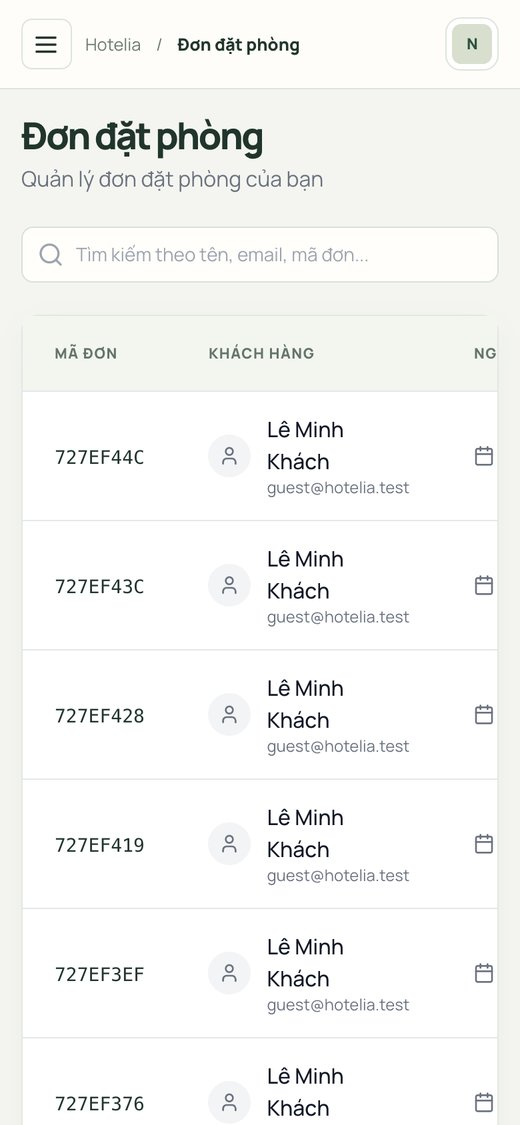
\includegraphics[height=7.5cm]{figures/shots/web-15-owner-bookings-mobile.jpg}}\hspace{1cm}
\subcaptionbox{Quản lý khách sạn, 768$\times$1024}{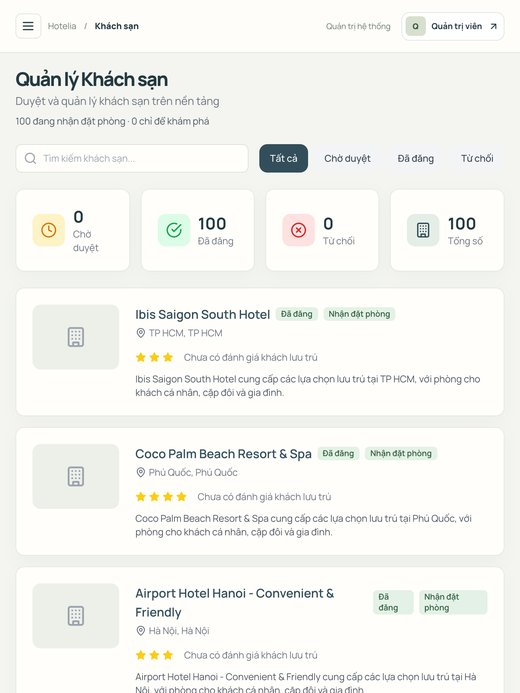
\includegraphics[height=7.5cm]{figures/shots/web-16-admin-hotels-tablet.jpg}}
\caption{Bảng điều khiển ở kích thước điện thoại và máy tính bảng}\label{fig:web-responsive}
\end{figure}

\section{Kiểm thử thành phần gợi ý}\label{sec:test-rec}

\subsection{Kiểm thử tự động}

\Cref{tab:test-rec} là các ca kiểm thử của thành phần gợi ý. Nhóm R01--R11 kiểm tra cách ly dữ liệu và ghi nhận tương tác. Nhóm R12--R13 kiểm tra cơ chế dự phòng. Nhóm R14--R17 kiểm tra khớp Python -- TypeScript. Nhóm R18--R22 kiểm tra bộ xếp hạng theo nội dung.

\begin{rtable}
\begin{longtable}{|C{1.2cm}|L{9.6cm}|C{1.6cm}|}
\caption{Ca kiểm thử thành phần gợi ý}\label{tab:test-rec}\\
\hline
\thead{Mã} & \thead{Kịch bản} & \thead{Kết quả} \\ \hline
\endfirsthead
\hline
\thead{Mã} & \thead{Kịch bản} & \thead{Kết quả} \\ \hline
\endhead
TC-R01 & Người dùng đăng nhập: chỉ dùng lịch sử \code{user:id}, không dùng \code{session} & Đạt \\ \hline
TC-R02 & Khách ẩn danh: không truy vấn đặt phòng của bất kỳ ai & Đạt \\ \hline
TC-R03 & Xếp hạng toàn bộ ứng viên trước khi cắt theo \code{limit} & Đạt \\ \hline
TC-R04 & Giữ bộ lọc điểm đến dù lịch sử nghiêng về thành phố khác & Đạt \\ \hline
TC-R05 & Mở lại cùng khách sạn không tăng số lượt xem & Đạt \\ \hline
TC-R06 & Lượt mở chỉ gắn vào lượt hiển thị khi đúng tác nhân, mã và ứng viên & Đạt \\ \hline
TC-R07 & Lượt hiển thị giữ thứ tự, tối đa 8, không bị ghi đè khi gửi lại & Đạt \\ \hline
TC-R08 & Từ chối ứng viên trùng hoặc chưa duyệt & Đạt \\ \hline
TC-R09 & Không lưu văn bản tìm kiếm tự do & Đạt \\ \hline
TC-R10 & Không gắn nhãn ``đã mở'' cho khách sạn không hiển thị hoặc người dùng khác & Đạt \\ \hline
TC-R11 & Xóa cả lượt xem và lượt hiển thị của một tác nhân & Đạt \\ \hline
TC-R12 & Mô hình không chấm được: dùng bộ xếp hạng nội dung, \code{modelUsed = false} & Đạt \\ \hline
TC-R13 & Mô hình chấm được: báo đúng \code{version}, \code{modelUsed = true} & Đạt \\ \hline
TC-R14 & Khớp điểm số Python -- TypeScript trên 5 véc-tơ (9 chữ số) & Đạt \\ \hline
TC-R15 & Khớp 16 đặc trưng trên 2 kịch bản, 8 khách sạn (9 chữ số) & Đạt \\ \hline
TC-R16 & Đặc trưng giờ theo giờ Việt Nam với \code{TZ=UTC} và \code{TZ=America/Los\_Angeles} & Đạt \\ \hline
TC-R17 & Nạp mô hình đang phục vụ và xếp hạng & Đạt \\ \hline
TC-R18 & Khởi động lạnh: đa dạng thành phố, không bịa đánh giá & Đạt \\ \hline
TC-R19 & Ưu tiên khách sạn tương tự về thành phố, tiện nghi, giá & Đạt \\ \hline
TC-R20 & Chuẩn hóa bí danh thành phố (TP HCM, Sài Gòn) và dấu & Đạt \\ \hline
TC-R21 & Một đánh giá 5 sao không vượt khách sạn có nhiều đánh giá tốt & Đạt \\ \hline
TC-R22 & Thiếu giá, không rõ hạng sao: không sinh NaN, không mất ứng viên & Đạt \\ \hline
\end{longtable}
\end{rtable}

\subsection{Tệp mô hình lỗi}

\Cref{tab:test-artifact} là kết quả khi cố ý làm hỏng tệp mô hình trong một bản sao của thư mục build. Trong mọi trường hợp lỗi, \code{rank} trả về \code{undefined}, nên API dùng bộ xếp hạng dự phòng; một cảnh báo cho biết nguyên nhân được ghi vào nhật ký. Trường hợp M5 cho thấy lỗi xuất hiện lúc chấm điểm (tệp nạp được nhưng cây hỏng) cũng được bắt.

\begin{table}[H]
\centering
\caption{Hành vi khi tệp mô hình bị lỗi}\label{tab:test-artifact}
\begin{rtable}
\begin{tabular}{|C{1.0cm}|L{3.6cm}|C{1.6cm}|L{3.2cm}|L{4.6cm}|}
\hline
\thead{Mã} & \thead{Tình huống} & \thead{Nạp được} & \thead{Xếp hạng} & \thead{Cảnh báo ghi nhận} \\ \hline
M1 & Tệp hợp lệ & có & LightGBM & -- \\ \hline
M2 & Không phải JSON & không & dự phòng & lỗi phân tích JSON \\ \hline
M3 & Đảo thứ tự đặc trưng & không & dự phòng & Model feature contract does not match backend \\ \hline
M4 & Không có cây & không & dự phòng & Model has no trees \\ \hline
M5 & Nút cây thiếu nhánh & có & dự phòng & Invalid LightGBM tree node \\ \hline
M6 & Tệp bị xóa & không & dự phòng & ENOENT \\ \hline
\end{tabular}
\end{rtable}
\end{table}

\section{Đánh giá mô hình LightGBM}\label{sec:eval-model}

\subsection{Thiết lập}

Ba phiên bản mô hình đã được huấn luyện. Cả ba dùng cùng 16 đặc trưng và mục tiêu LambdaRank, nhưng khác nhau về dữ liệu và cách đánh giá (\cref{tab:model-versions}). Mọi số liệu đều là đánh giá ngoại tuyến trên dữ liệu sinh trước phát hành, không phải số đo trên người dùng thật.

\begin{rtable}
\begin{longtable}{|L{3.8cm}|L{3.5cm}|L{3.5cm}|L{3.8cm}|}
\caption{Thiết lập của ba phiên bản mô hình}\label{tab:model-versions}\\
\hline
\thead{Khía cạnh} & \thead{v1 (23/10)} & \thead{v2 (23/10)} & \thead{v3 (24/10, đang phục vụ)} \\ \hline
\endfirsthead
\hline
\thead{Khía cạnh} & \thead{v1 (23/10)} & \thead{v2 (23/10)} & \thead{v3 (24/10, đang phục vụ)} \\ \hline
\endhead
Thuộc tính khách sạn & Sinh bằng hàm băm & Sinh bằng hàm băm & Ảnh chụp API (giá trị thật của danh mục) \\ \hline
Lịch sử mô phỏng & Một hồ sơ ưa thích cố định & Tín hiệu có trọng số như máy chủ, 1--12 tín hiệu & Như v2, 1--50 tín hiệu, 90 ngày \\ \hline
Nhóm ứng viên & 8 & 8 & 8; theo thành phố; toàn bộ 100 \\ \hline
Số truy vấn & 8.000 (6.800 / 1.200) & 8.000 (6.800 / 1.200) & 20.000 (14.000 / 3.000 / 3.000) \\ \hline
Tập báo cáo & Kiểm định (dùng cả để dừng sớm) & Kiểm định (dùng cả để dừng sớm) & Kiểm tra riêng \\ \hline
Đường cơ sở & quality\_prior & quality\_prior & quality\_prior, bộ xếp hạng nội dung, oracle \\ \hline
Giờ trong đặc trưng & Giờ của máy chủ & Giờ của máy chủ & Giờ Việt Nam \\ \hline
Số cây (best iteration) & 7 & 41 & 10 \\ \hline
\end{longtable}
\end{rtable}

\subsection{Kết quả}

\Cref{tab:model-results} tổng hợp kết quả của ba phiên bản. Với v1 và v2, mỗi truy vấn chỉ có 8 ứng viên, nên Hit@10 luôn bằng 1 kể cả với thứ tự ngẫu nhiên và không được dùng để so sánh.

\begin{table}[H]
\centering
\caption{Kết quả đánh giá ngoại tuyến các phiên bản mô hình}\label{tab:model-results}
\begin{rtable}
\begin{tabular}{|L{1.5cm}|L{4.1cm}|C{2.1cm}|C{2.1cm}|C{2.1cm}|L{2.4cm}|}
\hline
\thead{Phiên bản} & \thead{Phương pháp} & \thead{MRR@10} & \thead{NDCG@10} & \thead{Hit@10} & \thead{Tập đo} \\ \hline
\multirow{2}{*}{v1} & Đường cơ sở quality\_prior & 0,342 & 0,496 & 1,000 & \multirow{2}{*}{Kiểm định} \\ \cline{2-5}
 & LightGBM & 0,620 & 0,713 & 1,000 & \\ \hline
\multirow{2}{*}{v2} & Đường cơ sở quality\_prior & 0,373 & 0,520 & 1,000 & \multirow{2}{*}{Kiểm định} \\ \cline{2-5}
 & LightGBM & 0,539 & 0,650 & 1,000 & \\ \hline
\multirow{4}{*}{v3} & Đường cơ sở quality\_prior & 0,286 & 0,405 & 0,796 & \multirow{4}{2.4cm}{Kiểm tra, 3.000 truy vấn} \\ \cline{2-5}
 & Bộ xếp hạng nội dung (dự phòng) & 0,416 & 0,526 & 0,879 & \\ \cline{2-5}
 & LightGBM & 0,415 & 0,524 & 0,871 & \\ \cline{2-5}
 & Oracle (lợi ích kỳ vọng, không nhiễu) & 0,424 & 0,534 & 0,884 & \\ \hline
\end{tabular}
\end{rtable}
\end{table}

\Cref{tab:model-groups} chia kết quả v3 theo loại nhóm ứng viên. Nhóm \code{full\_catalog} (100 ứng viên) là nơi Hit@10 có ý nghĩa, vì chỉ 10\% ứng viên lọt vào top 10.

\begin{table}[H]
\centering
\caption{MRR@10 của v3 theo loại nhóm ứng viên (tập kiểm tra)}\label{tab:model-groups}
\begin{rtable}
\begin{tabular}{|L{2.8cm}|C{1.5cm}|C{1.8cm}|C{1.8cm}|C{1.9cm}|C{2.1cm}|C{1.6cm}|}
\hline
\thead{Nhóm} & \thead{Truy vấn} & \thead{Ứng viên TB} & \thead{Quality} & \thead{Nội dung} & \thead{LightGBM} & \thead{Oracle} \\ \hline
sample\_8 & 1.311 & 8 & 0,335 & 0,519 & 0,529 & 0,537 \\ \hline
destination & 1.106 & 8,8 & 0,363 & 0,414 & 0,407 & 0,414 \\ \hline
full\_catalog & 583 & 100 & 0,029 & 0,190 & 0,176 & 0,191 \\ \hline
\multicolumn{3}{|l|}{Hit@10 của nhóm full\_catalog} & 0,084 & 0,458 & 0,419 & 0,480 \\ \hline
\end{tabular}
\end{rtable}
\end{table}

\subsection{Phân tích}

\paragraph{Chênh lệch lớn ở v1, v2 đến từ cách đánh giá.} Ở v1 và v2, LightGBM hơn đường cơ sở 0,17--0,28 điểm MRR. Tuy nhiên đường cơ sở đó là \code{quality\_prior}, chỉ xét chất lượng khách sạn và hoàn toàn bỏ qua lịch sử. Trong khi đó, nhãn được sinh chủ yếu từ độ phù hợp với lịch sử (hệ số của \code{city\_affinity} là 1,75 so với 0,7 của \code{quality\_prior}). Một mô hình chỉ cần học ``ưu tiên khách sạn cùng thành phố với lịch sử'' là đã vượt đường cơ sở này. Ngoài ra, số liệu được báo cáo trên chính tập dùng để chọn số cây, nên có thiên lệch lạc quan nhỏ. Kết quả của v1 cao hơn v2 cũng không có nghĩa v1 tốt hơn: dữ liệu v1 dùng một hồ sơ ưa thích cố định, tạo ra quan hệ đơn giản hơn giữa đặc trưng và nhãn.

\paragraph{Với v3, LightGBM ngang bộ xếp hạng nội dung.} Khi so với bộ xếp hạng nội dung, tức chính cơ chế dự phòng của hệ thống, LightGBM v3 đạt MRR@10 0,415 so với 0,416. Chênh lệch này không đáng kể. LightGBM nhỉnh hơn ở nhóm 8 ứng viên (0,529 so với 0,519) nhưng kém hơn ở nhóm 100 ứng viên (0,176 so với 0,190). Cả hai đều rất gần mức oracle 0,424. Mức oracle là thứ tự theo đúng hàm lợi ích dùng để sinh nhãn, nên là giới hạn trên mà không mô hình nào vượt được trên tập dữ liệu này.

\paragraph{Vì sao mức trần thấp.} Oracle chỉ đạt 0,424 vì nhãn có nhiễu Gumbel: ngay cả khi biết chính xác lợi ích kỳ vọng, khách sạn tốt nhất cũng chỉ được chọn với một xác suất nhất định. Điều này mô phỏng việc người dùng thật không luôn chọn phương án ``tối ưu''.

\paragraph{Vì sao LightGBM không vượt bộ xếp hạng nội dung.} Hàm sinh nhãn là tổ hợp tuyến tính của các đặc trưng gần giống công thức của bộ xếp hạng nội dung: cùng thành phố, giá, sao, tiện nghi, chất lượng. Dữ liệu vì vậy không chứa quy luật nào mà công thức viết tay chưa nắm được. Mức độ quan trọng của đặc trưng (\cref{fig:importance}) xác nhận điều này. \code{city\_affinity} chiếm 44,6\% tổng độ lợi; tiếp theo là \code{price\_relative} 13,9\% và \code{price\_affinity} 12,8\%. Các đặc trưng thời gian gần như không được dùng: \code{hour\_sin} 0,5\%, \code{is\_weekend} 0\%. Kết quả này phù hợp với việc hàm sinh nhãn chỉ cộng 0,12 cho tiện nghi gia đình vào cuối tuần.

\begin{figure}[H]
\centering
\diagram{importance}
\caption{Tỷ lệ độ lợi (gain) của từng đặc trưng trong mô hình v3}\label{fig:importance}
\end{figure}

\paragraph{Kết luận về mô hình.} Các thực nghiệm chứng minh được bốn điều: (i) đường ống huấn luyện -- xuất -- phục vụ hoạt động đầu-cuối; (ii) mã TypeScript tái hiện chính xác điểm số và đặc trưng của Python; (iii) mô hình học được quy luật có trong dữ liệu, sát giới hạn trên; (iv) cơ chế dự phòng hoạt động khi mô hình lỗi. Các thực nghiệm không chứng minh rằng LightGBM gợi ý tốt hơn bộ xếp hạng nội dung, cũng không chứng minh rằng gợi ý làm tăng tỷ lệ đặt phòng của người dùng thật. Hai kết luận đó chỉ có thể rút ra từ dữ liệu hành vi thật và thử nghiệm A/B (\cref{sec:future}).

\subsection{Thí nghiệm phụ trên dữ liệu Trivago}\label{sec:trivago}

Trước khi xây dựng mô hình cho danh mục Hotelia, đồ án thử LambdaRank trên bộ dữ liệu Trivago RecSys Challenge 2019 \cite{adamczak2019} để kiểm tra phương pháp trên hành vi thật. Mỗi lượt bấm vào khách sạn (clickout) là một truy vấn; các khách sạn trong danh sách hiển thị là ứng viên. 18 đặc trưng chỉ dùng thông tin có trước lượt bấm (vị trí, giá, thứ hạng giá, tương tác trước đó trong phiên, thiết bị, giờ). Mô hình huấn luyện trên mẫu 100.000 hành động đầu tiên, chọn số cây trên 15\% phiên mới nhất của tập huấn luyện, rồi đánh giá trên một tập thời gian muộn hơn.

\begin{table}[H]
\centering
\caption{Kết quả thí nghiệm phụ trên Trivago RecSys 2019 (tập thời gian muộn hơn)}\label{tab:trivago}
\begin{rtable}
\begin{tabular}{|L{6.8cm}|C{2.0cm}|C{2.0cm}|C{2.0cm}|C{1.8cm}|}
\hline
\thead{Phương pháp} & \thead{MRR@10} & \thead{NDCG@10} & \thead{Hit@10} & \thead{Truy vấn} \\ \hline
B0: giữ thứ tự hiển thị gốc & 0,389 & 0,472 & 0,744 & 7.055 \\ \hline
B1: tần suất bấm theo (thành phố, khách sạn) & 0,313 & 0,412 & 0,737 & 7.068 \\ \hline
B2: độ phổ biến thành phố + số tiện nghi & 0,263 & 0,343 & 0,607 & 7.068 \\ \hline
LightGBM LambdaRank (B6, 43 cây) & 0,521 & 0,597 & 0,842 & 7.055 \\ \hline
\end{tabular}
\end{rtable}
\end{table}

Trên hành vi thật của Trivago, LightGBM hơn thứ tự hiển thị gốc 0,13 điểm MRR@10 (\cref{tab:trivago}). Kết quả này cho thấy phương pháp có giá trị khi dữ liệu chứa quy luật thật. Tuy nhiên, mô hình này không thể dùng cho Hotelia: mã khách sạn Trivago không ánh xạ được sang danh mục Hotelia, và đặc trưng được mô hình dùng để chia nút nhiều nhất (206 lần) là vị trí trong danh sách hiển thị gốc của Trivago, vốn không tồn tại trong Hotelia.

\section{Đánh giá chung}\label{sec:overall}

\subsection{Kết quả đạt được và ưu điểm}

\begin{itemize}
\item Tính đúng của đặt phòng được kiểm chứng trên cơ sở dữ liệu thật. Tình huống hai khách tranh căn phòng cuối, thử lại, hết hạn giữ và hủy được kiểm tra bằng giao dịch MongoDB thật, không chỉ bằng mô hình giả lập.
\item Bảo mật theo nguyên tắc ``không tin máy khách''. Số tiền thanh toán, trạng thái thanh toán, vai trò và quyền sở hữu đều được quyết định ở máy chủ. Quá trình kiểm tra lại khi viết báo cáo phát hiện và sửa một lỗ hổng thật (refresh token dùng như access token).
\item Gợi ý chạy trong cùng tiến trình, có dự phòng và có kiểm thử khớp. Không cần thêm dịch vụ, độ trễ mạng hay chi phí vận hành. Mọi lỗi của mô hình đều được chuyển sang dự phòng.
\item Trung thực về dữ liệu. Giao diện phân biệt điểm biên tập với đánh giá đã xác minh; báo cáo phân biệt dữ liệu thật với dữ liệu mô phỏng.
\item Triển khai thật. API, bảng điều khiển và cơ sở dữ liệu đang chạy với tên miền \code{hotelia.asia}; việc cập nhật mô hình có quy trình và đã được thực hiện.
\end{itemize}

\subsection{Giới hạn}\label{sec:limitations}

\begin{rtable}
\begin{longtable}{|C{0.7cm}|L{4.2cm}|L{9.8cm}|}
\caption{Các giới hạn của hệ thống}\label{tab:limitations}\\
\hline
\thead{\#} & \thead{Giới hạn} & \thead{Mô tả và hệ quả} \\ \hline
\endfirsthead
\hline
\thead{\#} & \thead{Giới hạn} & \thead{Mô tả và hệ quả} \\ \hline
\endhead
1 & Dữ liệu huấn luyện là dữ liệu sinh & Nhãn đến từ hàm lợi ích giả định; mô hình chưa học từ hành vi thật. Chưa có A/B test. Không thể kết luận về hiệu quả trên người dùng. \\ \hline
2 & Danh mục mô phỏng một phần & 80/100 khách sạn có giá, tồn kho, chủ khách sạn sinh tự động; điểm đánh giá là dữ liệu biên tập; số đánh giá đã xác minh trên môi trường vận hành bằng 0. \\ \hline
3 & Chưa có hoàn tiền tự động & \code{refund} trả 503; \code{calculateRefund} chưa được dùng; đặt phòng đã thanh toán payOS không thể xác nhận hủy qua hệ thống. \\ \hline
4 & payOS chưa kiểm thử với giao dịch thật & Chỉ có kiểm thử đơn vị với khóa thử; chưa có bằng chứng giao dịch thành công trên môi trường vận hành. \\ \hline
5 & Trạng thái chưa dùng & PAID, REFUNDED, COMPLETED được khai báo nhưng chưa có luồng; bảng \code{roomavailabilities} còn trong mã nhưng không dùng. \\ \hline
6 & Sign in with Apple phụ thuộc tài khoản trả phí & Bản build với tài khoản miễn phí ẩn nút Apple; luồng Apple mới được kiểm thử ở mức đơn vị. \\ \hline
7 & Quên mật khẩu phụ thuộc dịch vụ email & Cần cấu hình \code{RESET\_EMAIL\_WEBHOOK\_URL}; nếu chưa cấu hình, chức năng trả 503. \\ \hline
8 & Bảng điều khiển chỉ có tiếng Việt & Chưa có i18n cho web; nội dung dữ liệu chủ yếu tiếng Việt. \\ \hline
9 & Hạ tầng gói miễn phí & Render tạm dừng khi không có lưu lượng; yêu cầu đầu tiên có thể chờ hơn 20 giây. Chưa có giám sát, cảnh báo, sao lưu được cấu hình trong mã. \\ \hline
10 & Chưa kiểm thử tải và kiểm thử giao diện tự động & Chưa đo thông lượng, độ trễ dưới tải; chưa có XCUITest, Playwright. \\ \hline
11 & Chưa có cơ chế xin đồng ý thu thập dữ liệu & Dữ liệu tương tác được tối thiểu hóa và tự xóa, nhưng chưa có màn hình xin đồng ý theo Nghị định 13/2023/NĐ-CP. \\ \hline
\end{longtable}
\end{rtable}

\subsection{Rủi ro}

\begin{itemize}
\item Rủi ro vận hành thanh toán: nếu địa chỉ webhook bị chặn hoặc máy chủ đang ngủ khi payOS gửi webhook, đặt phòng có thể hết hạn giữ dù khách đã trả tiền. Hệ thống đã xử lý tình huống tiền về sau hạn bằng cách chuyển sang CANCEL\_REQUESTED, nhưng việc hoàn tiền vẫn phải làm thủ công.
\item Rủi ro dữ liệu: catalog thay đổi (giá, khách sạn mới) mà không huấn luyện lại sẽ làm phân phối đặc trưng lúc phục vụ lệch dần khỏi lúc huấn luyện.
\item Rủi ro bảo mật: refresh token cũ (không có \code{typ}) còn được chấp nhận tới khi hết hạn 7 ngày sau bản sửa. Mỗi tài khoản chỉ giữ một refresh token, nên đăng nhập trên thiết bị thứ hai làm phiên trên thiết bị thứ nhất hết hiệu lực khi access token hết hạn.
\end{itemize}

\section{Hướng phát triển}\label{sec:future}

\begin{enumerate}
\item Dữ liệu hành vi thật có đồng thuận. Bổ sung màn hình xin đồng ý thu thập dữ liệu tương tác cho mục đích gợi ý, cho phép rút lại đồng ý; dùng lượt hiển thị, lượt mở chi tiết, giữ phòng và đặt phòng đã xác nhận làm nhãn nhiều mức (ví dụ mở = 1, giữ = 2, xác nhận = 3). Cần hiệu chỉnh thiên lệch vị trí khi học từ nhật ký \cite{joachims2017}.
\item Thử nghiệm A/B. Chia ngẫu nhiên người dùng giữa bộ xếp hạng nội dung và LightGBM. Chỉ số chính là tỷ lệ đặt phòng được xác nhận trên mỗi lượt hiển thị; chỉ số bảo vệ là tỷ lệ hủy và độ trễ phản hồi \cite{kohavi2009}. Chỉ bật mô hình cho toàn bộ người dùng khi chênh lệch có ý nghĩa thống kê.
\item Giám sát mô hình và hệ thống. Ghi \code{ranking.mode} và \code{version} của mỗi phản hồi để theo dõi tỷ lệ rơi về dự phòng; theo dõi phân phối đặc trưng để phát hiện lệch; giám sát sức khỏe API, lỗi 5xx và thời gian phản hồi; nâng cấp gói hạ tầng để tránh khởi động lạnh.
\item Kho đặc trưng (feature store). Khi số khách sạn và người dùng tăng, tính sẵn các đặc trưng theo khách sạn và theo người dùng, dùng chung cho huấn luyện và phục vụ để loại bỏ lệch về định nghĩa.
\item Thanh toán trực tuyến đầy đủ. Cấu hình khóa payOS trên môi trường vận hành, kiểm thử bằng giao dịch thật giá trị nhỏ, cài đặt hoàn tiền theo \code{calculateRefund} với đối soát, và chuyển trạng thái REFUNDED.
\item Tối ưu tập ứng viên. Với danh mục lớn, thêm giai đoạn lọc thô (ví dụ theo khoảng cách, giá, độ phổ biến) để chỉ chấm điểm vài trăm ứng viên; lưu đệm danh mục đã lọc.
\item Đa dạng hóa kết quả. Áp dụng xếp hạng lại theo độ đa dạng (thành phố, mức giá, loại hình) cho cả đầu ra của LightGBM, không chỉ cho bộ xếp hạng dự phòng \cite{carbonell1998}.
\item Bảo mật môi trường vận hành. Hỗ trợ nhiều refresh token theo thiết bị kèm phát hiện tái sử dụng; thu hồi chủ động token cũ không có \code{typ}; chuyển refresh token trên web sang cookie \code{HttpOnly}; bổ sung giới hạn tần suất riêng cho \code{/auth}; quét phụ thuộc định kỳ; đối chiếu với OWASP ASVS \cite{owaspasvs}.
\item Hoàn thiện sản phẩm. Bản tiếng Anh cho bảng điều khiển; dịch nội dung khách sạn; trạng thái COMPLETED tự động sau khi trả phòng; thông báo đẩy; phát hành TestFlight; kiểm thử giao diện tự động; thay chuyển hướng ở \code{hotelia.asia} bằng trang giới thiệu sản phẩm.
\end{enumerate}

\section{Kết luận chương}

Chương này đã trình bày kết quả của 57 ca kiểm thử máy chủ, 80 ca kiểm thử Python, kịch bản tranh chấp trên MongoDB thật, 13 ca phân quyền và 7 ca phiên đăng nhập qua HTTP, 6 kịch bản lỗi mô hình và 18 ca kiểm thử giao diện. Quá trình kiểm thử phát hiện và sửa năm lỗi giao diện cùng một lỗ hổng xác thực. Đánh giá mô hình cho thấy LightGBM v3 học sát giới hạn của dữ liệu sinh nhưng không vượt bộ xếp hạng nội dung. Vì vậy đánh giá ngoại tuyến hiện tại chỉ xác nhận tính đúng của đường ống, chưa xác nhận hiệu quả gợi ý.
